%; whizzy chapter
% -initex iniptex -latex platex -format platex -bibtex jbibtex -fmt fmt
% 以上 whizzytex を使用する場合の設定。

%     Kansai Debian Meeting resources
%     Copyright (C) 2007 Takaya Yamashita
%     Thank you for Tokyo Debian Meeting resources

%     This program is free software; you can redistribute it and/or modify
%     it under the terms of the GNU General Public License as published by
%     the Free Software Foundation; either version 2 of the License, or
%     (at your option) any later version.

%     This program is distributed in the hope that it will be useful,
%     but WITHOUT ANY WARRANTY; without even the implied warranty of
%     MERCHANTABILITY or FITNESS FOR A PARTICULAR PURPOSE.  See the
%     GNU General Public License for more details.

%     You should have received a copy of the GNU General Public License
%     along with this program; if not, write to the Free Software
%     Foundation, Inc., 51 Franklin St, Fifth Floor, Boston, MA  02110-1301 USA

%  preview (shell-command (concat "evince " (replace-regexp-in-string "tex$" "pdf"(buffer-file-name)) "&"))
% 画像ファイルを処理するためにはebbを利用してboundingboxを作成。
%(shell-command "cd image200708; ebb *.png")

%%ここからヘッダ開始。

\documentclass[mingoth,a4paper]{jsarticle}
\usepackage{kansaimonthlyreport}
\usepackage[dvips]{xy}
\usepackage{ulem}

% 日付を定義する、毎月変わります。
\newcommand{\debmtgyear}{2013}
\newcommand{\debmtgdate}{25}
\newcommand{\debmtgmonth}{8}
\newcommand{\debmtgnumber}{75}

\begin{document}

\begin{titlepage}

% 毎月変更する部分、本文の末尾も修正することをわすれずに

 第\debmtgnumber{}回 関西 Debian 勉強会資料

\vspace{2cm}

\begin{center}
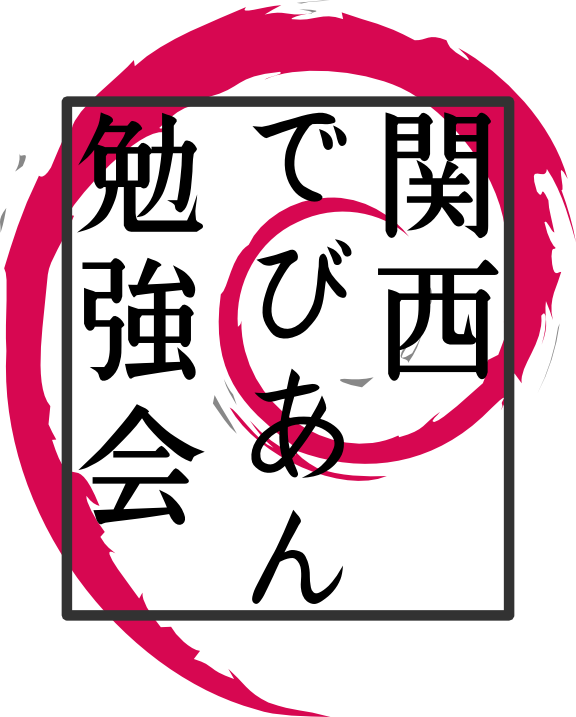
\includegraphics{image200802/kansaidebianlogo.png}
\end{center}

\begin{flushright}
\hfill{}関西 Debian 勉強会担当者 佐々木・倉敷・のがた・かわだ・八津尾 \\
\hfill{}\debmtgyear{}年\debmtgmonth{}月\debmtgdate{}日
\end{flushright}

\thispagestyle{empty}
\end{titlepage}

\dancersection{Introduction}{Debian JP}

\vspace{1em}

 関西Debian勉強会はDebian GNU/Linuxのさまざまなトピック
 (新しいパッケージ、Debian特有の機能の仕組、Debian界隈で起こった出来事、
 などなど)について話し合う会です。

 目的として次の三つを考えています。
 \begin{itemize}
  \item MLや掲示板ではなく、直接顔を合わせる事での情報交換の促進
  \item 定期的に集まれる場所
  \item 資料の作成
 \end{itemize}

 それでは、楽しい一時をお過ごしください。

\newpage

\begin{minipage}[b]{0.2\hsize}
 {\rotatebox{90}{\fontsize{80}{80}
{\gt 関西 Debian 勉強会}}}
\end{minipage}
\begin{minipage}[b]{0.8\hsize}
\hrule
\vspace{2mm}
\hrule
\setcounter{tocdepth}{1}
\tableofcontents
\vspace{2mm}
\hrule
\end{minipage}

\dancersection{最近のDebian関係のイベント報告}{Debian JP}

\subsection{大統一 Debian 勉強会 2013}
6 月 29 日(土)、日本大学駿河台キャンパスにて大統一 Debian 勉強会 2013
が開催されました。

全国各地の Debian 勉強会関係者と Debian に興味のある人達が一堂に会する
このイベント、2 回目となる今回は 140 名ほどの方々に参加していただきま
した。

イベントの模様は写真とともにレポートがあがっていますのでみてください。
\footnote{\url{http://gum.debian.or.jp/2013/blog/13-07-03}}
\footnote{\url{http://gihyo.jp/news/report/2013/07/1801}}

\subsection{関西 Debian 勉強会}
\subsubsection{第 72 回関西 Debian 勉強会}

72 回目の関西 Debian 勉強会は 5 月 26 日(日)に、ANNAI さんの協力のもと、
グランフロント大阪のナレッジサロンで行なわれました。
新しい話題の施設ですごく綺麗なところでした。

セッションは倉敷さんによる「Debian の歩き方」と西田さんの「Debian と
Ubuntu の違いを知ろう」の二本でした。

Debian のちょっとした使い方、Ubuntu との違いの理解が深められたのではな
いでしょうか。

\subsubsection{第 74 回関西 Debian 勉強会}
74 回目の関西 Debian 勉強会は 8 月 3 日(土)、京都リサーチパークで行なわ
れた OSC 2013 Kansai@Kyoto での出張版として行なわれました。

当日は「Debian 7.0 の実情/今後の開発について」としてセッションを開催し、
Raspberry Pi と MK802 の実機展示と Wheezy ライブイメージ配布などのブー
ス出展を行ないました。

\subsection{東京エリア Debian 勉強会}
\subsection{第 102 回東京エリア Debian 勉強会}
102 回目の東京エリア Debian 勉強会は 7 月 20 日(土)にあんさんぶる荻窪で
開催されました。

セッションは、岩松さんによる Debian Linux Kernel に追加された armmp フ
レーバーについて「Debian linux kernel / armmp フレーバー」と、Debian か
らみた Raspberry Pi として上川さんによる「Raspberry Pi を使ってみた」、そし
て「月刊 Debhelper」は野島さんが dh\_strip についてといった内容でした。

\subsection{第 103 回東京エリア Debian 勉強会}
103 回目の東京エリア Debian 勉強会は 8 月 17 日(土)にあんさんぶる荻窪で
開催されました。

セッションは、上川さんによる「OpenVPN を使ってみた」とまえださんによる
「Debian勉強会の資料のePUB化を試みた」の二本でした。

\subsection{Debian Project}

DebConf 13 が 8 月 11 日から 18 日にかけてスイスのヴォーマルキュで開催
されました。\footnote{\url{http://debconf13.debconf.org/}}

systemd、upstart の init システム、Google Compute Engine、AWS、OpenStack
などのクラウドと最近の話題のセッションが多く目につきました。「Ubuntu
daily quality improvements; overlap with Debian CUT」の CUT のセッショ
ンも気になりますね。

その他開催されたさまざまなセッションの模様は録画され配信されています。
\footnote{\url{http://penta.debconf.org/dc13_schedule/index.en.html}}

また、開催期間中の 8 月 16 日に Debian は誕生から 20 周年を迎え盛大に
パーティも開かれたようです。

来年の DebConf 14 はアメリカ、オレゴン州のポートランドで開催予定です。

一度は参加してみたいものですね。

\dancersection{事前課題}{Debian JP}

今回の課題は以下の通りです。
\begin{screen}
  \begin{enumerate}
  \item %
    構成管理システムをどのように活用(している/したい)かを記述してください
  \end{enumerate}
\end{screen}

参加者の皆さんの解答は以下の通りです:

\begin{prework}{ 川江 }
  \begin{enumerate}
  \item 取りあえず、sshd、bind、iptables、interfaces等々の設定の更新。synatpicの自動起動と自動アップデート。
  \item sshで家のサーバにログイン(Wheezyマシン)できるようにしときます。
  \end{enumerate}
\end{prework}

\begin{prework}{ かわにし }
  初参加です。

  構成管理システム自体良くわかりませんが、ぱっと思いついたのはサーバの構成でリソースをどれだけ使っていて、どうすれば改善されるかのヒントなどがでると初心者としては助かるなと思いました。
\end{prework}

\begin{prework}{ 山城の国の住人 久保博 }
  今まではサーバー管理はいくつか経験していたものの、今に至るまで構成管理システムを活用していません。

  これから仮想化環境が立てられるようなハードウェアを買って、仮想環境をたくさん飼えるようになりたいです。
\end{prework}

\begin{prework}{ かわだてつたろう }
  使ったことはありません。

  \begin{itemize}
  \item デプロイ先と同じ環境を容易に作りテストに使いたい。
  \item 設定の備忘録代わりにして環境移行(ハード交換、レンタルサーバ変更)のコストを下げられるとよいな。
  \end{itemize}
\end{prework}

\begin{prework}{ おくの }
  まだ使ったことがありません。ホスティングサーバ屋ですが、構成管理システム使ったら楽になれるならぜひ使いたいです。
\end{prework}

\begin{prework}{ 佐々木洋平 }
  構成管理のスクリプトはとくに使ったことはありません。50台ぐらいに対して clusterssh を使ってログインして、一括設定していたりします。あとは git で deploy する、とか。

  簡単にできたら良いな、とか思います。
\end{prework}

\begin{prework}{ kino }
  Q: 構成管理システムをどのように活用したいか

  A: 現状使えていないのですが希望としては、
  \begin{itemize}
  \item 開発サーバーとライブサーバーを同じ設定にして素早く立ちあげたい。
  \item Debianのアップグレードテスト環境を作りたい。
  \item 専用サーバーの上に仮想環境を作って、Vagrant+Puppetみたいな使い方をしたい。
  \end{itemize}
\end{prework}

\begin{prework}{ lurdan }
  小規模なデータセンターの管理に使っています。

  現状のメリット
  \begin{itemize}
  \item 共通設定について、一度対処したら忘れることができる
  \item イメージのクローンより、イレギュラー要望に対処しやすい
  \end{itemize}

  現状の課題
  \begin{itemize}
  \item 構成結果のテスト方法が確立できていない (serverspec と cucumber-nagios で模索中)
  \item 共通モジュールとしてくくり出す内容の線引きが悩ましい
  \end{itemize}
\end{prework}

\dancersection{puppet による構成管理の実践}{倉敷 悟}

\subsection{概要}

このセッションでは、まっさらな Wheezy 環境に puppet をセットアップし、
実際にマニフェストを書いて、Debian アーカイブの部分ミラーを構成させる
ところまで、実際に手を動かしながら実習していきます。

\subsection{完成図の検討}

まずは、構成管理としてやりたいことを検討します。今回のお題は、Debian
アーカイブの部分ミラーを構成する、ということになりますので、ざっくりと
下記のような構成で検討してみます。

\begin{itemize}
\item
  アーキテクチャは amd64 のみ
\item
  ディストリビューションは Wheezy (更新も含む)
\item
  とりあえず必要最低限 (required) のパッケージだけをミラーする
\item
  リポジトリの管理ツールとして reprepro を使う
\item
  puppet は reprepro の環境設定のみ行う。ミラー実行は (とりあえず) 手動
\item
  ミラーへのアクセスは http
\end{itemize}

細かいところは、多少は好みで変更してもらっても構いません。ただしミラー
対象を増やしたいのであれば、回線がリッチな時をおすすめします。

上記に付随して、

\begin{itemize}
\item
  Web サーバは apache2 を使う
\item
  Secure Apt のために GPG 設定が必要
\item
  配置場所は /var/www/debian で所有者 www-data にする
\end{itemize}

といったことも要件として検討しておく必要があります。

他にもあるかも知れませんが、おいおい加えていくこともできますので、
ひとまずこれくらいの想定で進めます。

\subsection{puppet のインストールと編集環境のセットアップ}

まずは、適当なファイルにマニフェストを書き殴りましょう。

今回、puppet はスタンドアローンでバッチ的に動作させる形で使います。
そのため、puppet のコマンドラインクライアントをインストールしてください。
また、構成管理する OS 上でマニフェストの操作も行いますので、好みの
テキストエディタをインストールします。emacs であれば、puppet-el
\footnote{vim の場合は vim-puppet} というパッケージを使うと、予約語の
色分けなどをしてくれるので便利です。
作業を記録するためにバージョン管理システムもインストールしておきましょう。

\begin{commandline}
sudo apt-get install puppet emacs puppet-el git tig

mkdir kdm201308
cd kdm201308
git init
\end{commandline}

\subsection{全体像を下書きしてみる}

最初に考えたおおよその完成イメージを実現するため、トップレベルのマニフェ
ストを「こう書けたら嬉しい」という感じで下書きしてみます。

先程作成しておいたディレクトリで、site.pp というファイルを編集して
いきます。

\begin{commandline}
mkdir manifests
emacs manifests/site.pp
\end{commandline}

\begin{commandline}
# 必要になりそうなパッケージを class として列挙
class {
  'apache2':;
  'reprepro':;
  'gnupg':;
}

# reprepro のミラーディレクトリをよしなに設定 (してほしい)
reprepro::mirror { '/var/www/debian':
  owner => 'www-data', group => 'www-data',
  architecture => 'amd64',
  distribution => 'wheezy',
  partial => 'required',
}

# apache のミラー公開用サイトを追加 (してほしい)
apache2::site {
  'mirror':
    content => '後で';
}
\end{commandline}

要するに、やりたいことは、

\begin{itemize}
\item reprepro でいい感じのミラーを作る
\item 作ったディレクトリを適当に Web アクセスできるようにする
\end{itemize}

ということですね。

とりあえず並べた class の要素はまだ存在しないため、このままでは
実行できません。それぞれ作ってあげる必要があります。

ひとまず、作業を git に入れておきましょう。ログは好きなように書いて
ください。

\begin{commandline}
git add site.pp
git commit
\end{commandline}

このあたりで、必要そうであれば、前回のおさらいも兼ねて puppet のマニフェスト
書式について口頭で簡単なおさらいをします。資料としては前回の分 (2010/06) を
参照してください。

\subsection{必要な class を作る}

さて、ここからが本番です。何はともあれ、不足している class 定義の枠と、
インストールするパッケージの指定だけしてみましょう。

\begin{commandline}
class apache2 {
  package { 'apache2':; }
}

class reprepro {
  package { 'reprepro':; }
}

class gnupg {
  package { 'gnupg':; }
}
\end{commandline}

これだけでも、とりあえず必要なパッケージは入ります。凝ってみたいなら、
リファレンスを見ながらパラメータを追加してみてもいいでしょう。

これだけでは、パッケージ固有の設定は debconf 任せになってしまいますので、
設定を追加するために、都合のよいリソース定義が必要になります。
まずは、全体像で書いたリソースを受ける枠をとりあえず作って……

\begin{commandline}
define reprepro::mirror (
  $owner,
  $group,
  $architecture,
  $distribution,
  $partial
  ) {

}

define apache2::site (
  $content
  ) {

}
\end{commandline}

それぞれの内部をどのように構成するか考えてみましょう。この
セッションでは、かなりやっつけ感の高い構成で流してしまいますが、
実際にマニフェストを書くときは、構成管理しようとしている対象の
パッケージの動きをしっかり観察するようにしてください。

ここにファイルを置くためには、このパッケージが入っていなくては
ならない、このファイルはこういうパーミッションで置かれている、
このリソースの後にこういう処理が必要だ、パッケージの削除が失敗
しないか、などなど……。\footnote{パッケージシステムとの整合を
とる話は、それだけでセッションが成立する程度にはトピックがある
ので、また別の機会に。}

構成管理をしっかり書こうと思えば、その対象をよく知っておく必要
があります。そこの手間が省けるツールではないので誤解のないように
しましょう。
ありもののレシピ使い回せばいいんじゃんウェーイ、という考え方も
ご時世としてはありなのかも知れませんが、その後の運用を誰かに
押しつけてトンズラできる環境でないのならばオススメしません。

さて、構成管理ツールが流行するよりも前から、dpkg はその一部を
担っているという経緯もありますので、

\begin{itemize}
\item 一部、やってることが puppet と被る(プロセスの起動制御など)
\item 設定方針が debian policy で決まっているため、やりたい設定と矛盾す
る場合がある
\end{itemize}

といったあたりに注意して、設定を煮詰めていきましょう。

\subsubsection{apache2}

実は、今回はいろいろな前提の上にのっかっているため、apache2 に
追加の設定は不要です。デフォルトのままで、reprepro によって作成
されるミラーにそのままアクセスできるはずです。

ただ、それだとさすがに味気ないですから、簡単にサイト設定の仕組みを
追加してみましょう。これは Debian においては、
/etc/apache2/sites-\{enabled$|$available\}/ ディレクトリと
a2ensite/a2dissite コマンドによって制御されている部分ですね。

きっちり書くなら、available ディレクトリに file リソースの content で
ファイルを配置し、ensure パラメータの内容によって enable/disable を制御
する exec リソースを書いておく、といったことをすればいいと思います。
ただし、今回は面倒なので単純に「content の内容を直接 sites-enabled に
つっこむ」だけにしておきます。

すると、おおよそ次のようになるかと思います。

\begin{commandline}
define apache2::site (
  $content
  ) {

  file { "/etc/apache2/sites-enabled/${name}":
    content => $content,
    require => Package['apache2'],
    notify  => Service['apache2'],
  }
}
\end{commandline}

設定ファイルを変更したら、プロセスも再起動して欲しいので、notify
も追加しました。この Service はまだ定義していないので、class の方に
対応する定義を書いておきましょう。

\begin{commandline}
class apache2 {
  package { 'apache2':; }
  service { 'apache2':; }
}
\end{commandline}

これで、apache2 の
\begin{itemize}
\item パッケージを入れ
\item 適当なサイト設定を行い
\item サービスを起動する
\end{itemize}
簡単な class が出来ました。

後は、実際に流しこむサイト設定を用意する必要があります。今回は、さきほど
書いたようにデフォルトのままでも動くので、そのままデフォルト設定をパクっ
ておくことにします。

一度 apache2 パッケージをインストールし、sites-available/default
ファイルをコピーしましょう。

\begin{commandline}
sudo apt-get install apache2
cp /etc/apache2/sites-available/default site-mirror.erb
sudo apt-get purge apache2 && sudo apt-get autoremove
\end{commandline}

このファイルをテンプレートとして content に渡してあげたいので、
所定の場所に配置した上で、マニフェストから読みこむようにして
おきます。
\begin{commandline}
mkdir templates
mv site-mirror.erb  templates

apache2::site {
  'mirror':
    content => template('site-mirror.erb');
}
\end{commandline}

これで、apache2 については一応完成です。このあたりで、git commit して
おきましょう。

パラメータの渡し方、ファイルの指定方法などは、選択肢がいくらでも
あって、正解はありません。かけられる時間や、どれくらい類似度の高い
構成を繰り返すのか、などマニフェストを作成する状況にあわせて調整
するようにしてください。\footnote{実例としてあげている処理は、考慮
の足りない、ダメなやっつけ仕事の例ですので、反面教師として頂ければ……}

\subsubsection{reprepro}

今回は reprepro 自体の使い方は主眼ではないので、簡単に紹介だけしておきます。

reprepro は、指定したディレクトリに Debian のミラーを構成するツールです。
指定ディレクトリに決まったフォーマットで設定ファイルを用意しておけば、
柔軟にミラーを構成できます。そのため、ちょっと手元でとか社内利用などの
用途で、気軽にミラーを用意することができます
\footnote{パブリックなフルミラーを用意したい場合は、別途専用のツールがあります}。

イメージできるほど対象のソフトウェアに馴染んでいない場合は、まず puppet
抜きで動作させてみて、挙動を把握するようにしましょう。ともあれ、手動で
reprepro をインストールします。

\begin{commandline}
sudo apt-get install reprepro
\end{commandline}

reprepro を動作させるために、conf/distributions と conf/updates、2 つの
設定ファイルが必要になります。
ミラーのファイル置き場にするディレクトリに移動してください。ここでは、
wheezy の部分ミラーを作成しますので、ひとまず下記の内容でファイルを
作成しましょう。

distributions には、公開する対象 (sources.list でディストリビューション
コードネームとして参照されるもの) を指定します。今回の例では wheezy と
なります。

\begin{commandline}
Codename: wheezy
Architectures: amd64
Description: wheezy-mirror
Components: main contrib
Update: wheezy wheezy-updates wheezy-security
\end{commandline}

updates には、ミラーに含めるパッケージを取得してくる上流のリポジトリを
指定します。

\begin{commandline}
Name: wheezy
Method: http://ftp.jp.debian.org/debian
Suite: wheezy
Components: main contrib
Architectures: amd64
VerifyRelease: AED4B06F473041FA
FilterFormula: Priority (==required)

Name: wheezy-updates
Method: http://ftp.jp.debian.org/debian
Suite: wheezy-updates
Components: main contrib
Architectures: amd64
VerifyRelease: AED4B06F473041FA
FilterFormula: Priority (==required)

Name: wheezy-security
Method: http://security.debian.org/debian-security
Suite: wheezy/updates
VerifyRelease: AED4B06F473041FA
FilterFormula: Priority (==required)
\end{commandline}

Secure APT 用の公開鍵は、次のようにしてインポートしておきます。

\begin{commandline}
gpg --recv-key AED4B06F473041FA
\end{commandline}

これによって、このミラーが上流からダウンロードする時に、公開鍵に
よる確認が行なわれます。

設定が終わったら、正しく動作するか確認します。

\begin{commandline}
reprepro -V update wheezy
\end{commandline}

少し時間がかかりますが、指定したミラーからファイルをダウンロードする
はずです。
終わったら、ノードの /etc/apt/souces.list を少しいじって、apt-get から
アクセスできるかどうか確認しておくといいでしょう。

さて、ここまでで reprepro が動作する設定ができあがりましたので、これを
puppet のマニフェストに移していきましょう。

一旦、reprepro で作成したファイル類を全て削除します(別にしなくても構い
ませんが、ここまでのテスト内容を掃除するためです)。

\begin{commandline}
rm -r /var/www/debian
\end{commandline}

先程作成した site.pp を開き、設定ファイルを流しこむ方法を考えます。
パラメータをテンプレートで受けるなど、やり方はいくつかありますが、ここでは
単純に、ファイルをそのまま置くだけとしておきます。

ミラーは、配置するディレクトリを変更すれば、ノード内に複数作成することが
できる (べきな) ので、クラスではなく、リソースとして定義します。

\begin{commandline}
class reprepro {
  package { 'reprepro':; }
}

define reprepro::mirror (
  $distributions,
  $updates,
  ) {
  # ミラーの配置ディレクトリを作成する
  ## リソース名としてフルパスが渡されてくる想定
  file { "$name":
    ensure => directory,
  }
  -> file { "${name}/conf":
    ensure => directory,
  }
  -> file { # 設定ファイルの名前はパラメータとして受け取る
    "${name}/conf/distributions":
      content => $distributions;
    "${name}/conf/updates":
      content => $updates;
  }
}
\end{commandline}


パラメータ指定をやめてファイルを直接与えることにしたので、呼び出し元も
変更する必要があります。

\begin{commandline}
# reprepro をよしなに設定してほしい
reprepro::mirror { '/var/www/mirror':
  owner => 'www-data', group => 'www-data',
  distributions => '上で作成したファイルの内容をペースト
最後に改行が必要なので注意
',
  updates       => 'こちらも同様に
'
}
\end{commandline}

ここまでで、puppet を実行することで、reprepro の設定ファイルが準備され、
後はコマンドを実行するだけ、という状態になります。忘れないように、git commit
しておきましょう。

最終的には reprepro コマンドの実行も puppet にやらせるといいのですが、
話が広がってしまうので、今回はここまでとしておきます。

\subsection{マニフェストの適用とデバッグ}

さて、ここまでで作成したマニフェストを実行すると、

\begin{itemize}
\item apache2 がセットアップされて、ミラーのディレクトリが公開される
\item ミラーのディレクトリに reprepro の設定が用意される
\end{itemize}

はずですので、早速試してみましょう。まずは、dry run から。

\begin{commandline}
puppet apply -v /etc/puppet/manifests/site.pp --noop
\end{commandline}

スペルミスや、記号抜けなど、書式違いがあれば puppet が教えてくれますので、
出力内容を確認してみてください。

問題なさそうなら、$--$noop を削って、そのまま実行しましょう。

\subsection{マニフェストの整理}

puppet は、モジュールという単位でマニフェストを分割することができます。

今回は、さほど大きなマニフェストを書いているわけではないので、site.pp
だけでも十分見通しがききますが、1ファイルにダラダラ書いていくにも限度が
あります。ある程度大きく育ってきたら、マニフェストを分割しましょう。

もし実例が見たい、ということであれば、後半部分でやりますのでリクエストを
ください。

\subsubsection{パッケージモジュール}

モジュールをどういう単位で切り出すかは、個人の好みもあると思いますが、
ここではとっかかりとして「パッケージ単位」をおすすめしておきます。

では、パッケージに対応した puppet モジュールの置き場所を決めましょう。
例えば、

\begin{commandline}
mkdir -p /etc/puppet/modules/
\end{commandline}

などとします。このディレクトリ以下に、モジュール名のディレクトリを作成
していくことになりますが、Debian での利用を考えると、「ソースパッケージ名」
を使うといいでしょう (バイナリパッケージが細かく分割されていたりするので)。

例えば、apache2 のモジュールを作るのであれば、

\begin{commandline}
mkdir -p /etc/puppet/modules/apache2/manifests
emacs /etc/puppet/modules/apache2/manifests/init.pp
\end{commandline}

のようにします。「モジュール名/manifests/init.pp」はルールなので、別の
ファイル名にすることはできません。
とりあえず、先程作成した、apache2 クラスの内容をこちらに移動させてみて
ください。

パッケージモジュールの内容を決める上では、次のことに注意するといいでしょう。
\begin{itemize}
\item
  パッケージ固有の内容に絞り、サイト固有の設定は可能な限り含めない
\item
  後で再利用できるようにパラメータを決める
\end{itemize}

\subsubsection{サービスモジュール}

パッケージモジュールを切り離した後は、ノード/サイト固有の設定が
site.pp に残っている状態になっているはずです。そのうち、今作業している
ノードだけでなく別のノードでも再利用しそうなロール (うちでは Web サーバは
いつもこの設定で作るようにしてるんだ、とか) も、可能であればモジュールと
して切り出しておきましょう。

puppet から見ると、用途に関係なくモジュールはモジュールなのですが、
パッケージモジュールと区別するために、便宜的にサービスモジュールと呼んで
おきます。
puppet の書式ガイドライン的には、モジュール名として頭に s\_ をつける
ことになっています。

サービスモジュールはサイト固有の内容になりますので、パッケージモジュール
ほど境界を気にしなくてもいいでしょう。

例えば、部分ミラーのロールを作るのであれば、

\begin{commandline}
mkdir -p /etc/puppet/services/s_mirror/manifests
emacs /etc/puppet/services/s_mirror/manifests/init.pp
\end{commandline}

として、今回作成した reprepro の設定内容自体や、apache2 のサイト設定
などを放りこむところからはじめるといいと思います。

\subsection{ここからの育て方}

ひとまず、今回のセッションで Debian アーカイブのローカルミラーが
お手軽に作れるようになっているハズでので、次のステップとして、

\begin{itemize}
\item reprepro の設定ファイル指定がダサすぎるのでなんとかする
\item ローカルミラーを参照するように sources.list を設定する
\item ローカルミラーに独自パッケージを追加できるように reprepro の設定を追加する
\item 手動のままだった reprepro のコマンド実行をリソースに含める
\item reprepro のコマンド実行を cron に登録してみる
\item germinate を使って必要なパッケージを指定してミラーの対象にする
\end{itemize}

といった拡張からはじめていくと、とっかかりやすいのではないかと
思います。公式のリファレンスを眺めながら頑張ってみましょう。

\dancersection{今後の予定}{Debian JP}

\subsection{関西 Debian 勉強会}

次回、第 76 回関西 Debian 勉強会は 9 月 22 日(日)に港区民センターで開催予定です。

その前に、9 月 14 日(土)に札幌コンベンションセンターで開催される OSC 2013 Hokkaido に出張しセミナー発表を行ないます。

また、11 月は 11 月 8 日(金)、9 日(土)と大阪南港 ATC ITM 棟で開催される KOF2013 に出張予定です。


\subsection{東京エリア Debian 勉強会}

第 104 回東京エリア Debian 勉強会は 9 月 21 日(土)に開催予定です。

10 月は 10 月 19 日(土)、20 日(日)に行なわれる OSC 2013 Tokyo/Fall での出張開催予定です。

%
% 冊子にするために、4の倍数にする必要がある。
% そのための調整
 \dancersection{メモ}{}
 \mbox{}\newpage
 \mbox{}\newpage
 \mbox{}\newpage

\printindex
%\cleartooddpage

 \begin{minipage}[b]{0.2\hsize}
  \rotatebox{90}{\fontsize{80}{80} {\gt 関西 Debian 勉強会} }
 \end{minipage}
 \begin{minipage}[b]{0.8\hsize}

 \vspace*{15cm}
 \rule{\hsize}{1mm}
 \vspace{2mm}
 
\includegraphics[width=2cm]{image200502/openlogo-nd.eps}
 \noindent \Large \bf Debian 勉強会資料\\ \\
 \noindent \normalfont \debmtgyear{}年\debmtgmonth{}月\debmtgdate{}日 \hspace{5mm}  初版第1刷発行\\
 \noindent \normalfont 関西 Debian 勉強会 (編集・印刷・発行)\\
 \rule{\hsize}{1mm}
 \end{minipage}

\end{document}
